\section{Hardware}
\textbf{Arduino Uno:} The Arduino Uno is an open-source microcontroller board based on the ATmega328P, widely recognized for its simplicity, versatility, and ease of integration in embedded systems and prototyping applications. It features 14 digital input/output pins, 6 analog inputs, a 16 MHz quartz crystal, USB connection, power jack, and reset button, making it suitable for a broad range of hardware interfacing tasks. It's Von Neumann design integrates 32 KB flash memory, 2 KB SRAM, and 1 KB EEPROM, balancing program storage and runtime data handling. Native communication protocols (UART, I²C, SPI) enable efficient interfacing with IMUs (MPU6050) and wireless modules (ESP8266). Operating at 5V logic, its GPIO pins feature configurable pull-up resistors and interrupt support for real-time signal processing. The microcontroller executes firmware via polling or interrupts, translating raw inputs into processed outputs through timing-critical routines. This architecture ensures deterministic behavior, essential for low-latency gesture recognition systems where synchronized hardware-software interaction is paramount. 
 In this project, the Arduino Uno acts as the central processing unit that reads input data from multiple tactile switches and an MPU sensor, interprets the gestures or finger movements, and transmits the corresponding signals to the game engine. The board's real-time processing capability ensures minimal latency in interpreting physical gestures into digital commands. 
\begin{figure}[htbp!]
\centering
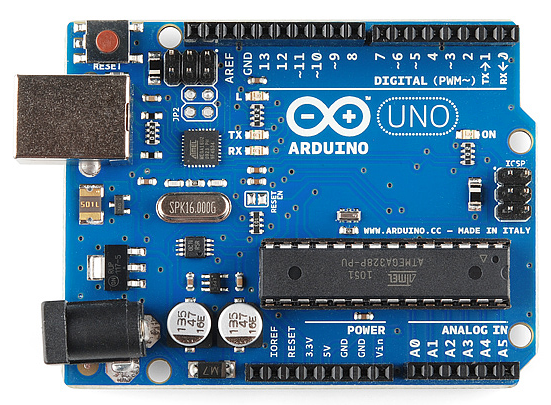
\includegraphics[width=0.5\textwidth]{images/fig3.1.png}
\caption{\textbf{Arduino Uno Board}}
\label{fig:3.1}
\end{figure}

\vspace{1.5\baselineskip} % Adds 1.5 line spaces before next section

\textbf{ESP8266}: The ESP8266 is a low-cost, high-performance Wi-Fi microcontroller based on a 32-bit RISC CPU core (Tensilica L106), operating at 80–160 MHz. It integrates TCP/IP protocol stack and supports IEEE 802.11 b/g/n standards, enabling wireless connectivity with low power consumption (~80 mA active mode). It enables devices to connect to wireless networks and communicate over the internet or within local networks. The ESP8266 supports multiple modes such as station, access point, and both simultaneously, making it highly versatile for wireless communication. It can be programmed using the Arduino IDE and is capable of handling HTTP requests, data transfer, and remote control functionalities. The ESP8266 is used to explore wireless communication possibilities between the hardware controller and the game system, potentially allowing untethered interaction.

\begin{figure}[htbp!]
\centering
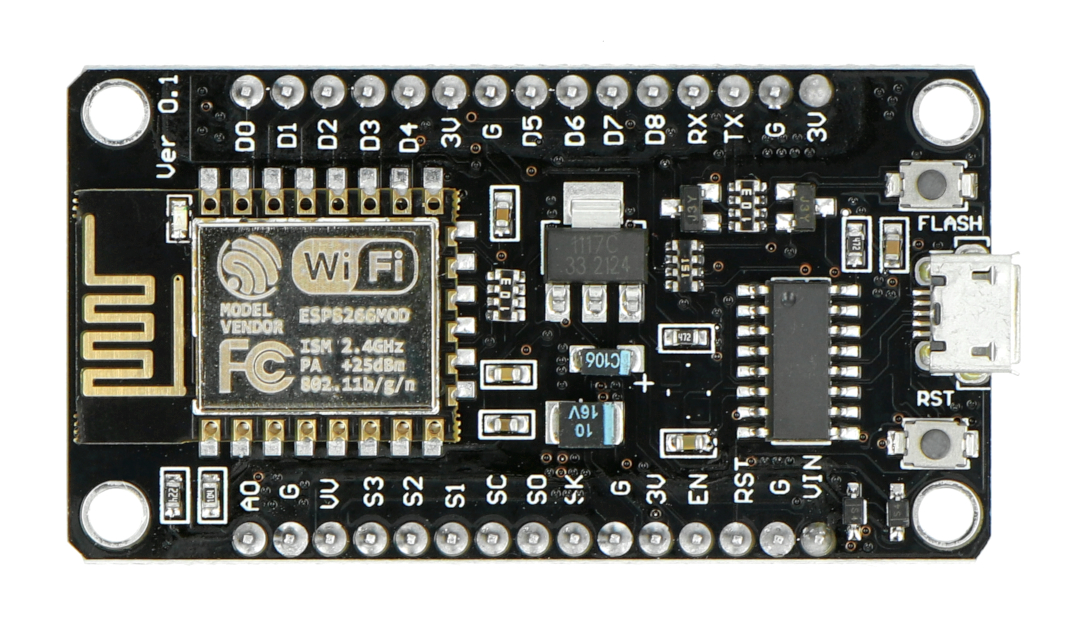
\includegraphics[width=0.5\textwidth]{images/fig3.2.jpg}
\caption{\textbf{ESP8266 Wi-Fi Module}}
\label{fig:3.2}
\end{figure}

\section{Software}
\lipsum[4-8]
%\section{Dataset}
%\lipsum[4-8]
